\documentclass[tikz,border=10pt]{standalone}
\usepackage{tkz-euclide} % 引入几何增强包逻辑

\begin{document}
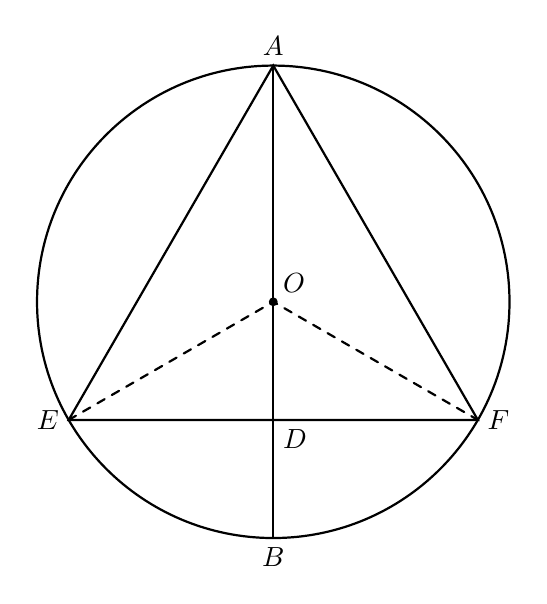
\begin{tikzpicture}[scale=2, line cap=round, line join=round，font=\large]
    % 1. 定义基本参数
    \def\R{1.5} % 圆半径
    \coordinate (O) at (0,0); % 圆心
    \coordinate (A) at (0,\R); % 顶点A
    \coordinate (B) at (0,-\R); % 底点B
    
    % 定义弦EF的位置（设D点在圆心下方0.5R处）
    \coordinate (D) at (0,-0.5*\R); 
    
    % 通过交点计算 E 和 F 的坐标
    % 弦EF所在的直线方程为 y = -0.5R
    \pgfmathsetmacro{\ex}{-sqrt(\R^2 - (0.5*\R)^2)}
    \coordinate (E) at (\ex, -0.5*\R);
    \coordinate (F) at (-\ex, -0.5*\R);

    % 2. 绘制图形
    % 绘制圆
    \draw[thick] (O) circle (\R);
    
    % 绘制直径 AB
    \draw[thick] (A) -- (B);
    
    % 绘制三角形 AEF 和 弦 EF
    \draw[thick] (A) -- (E) -- (F) -- cycle;
    \draw[dashed,thick] (E)--(O)--(F);

    % 3. 标注特殊点（圆心O）
    \fill (O) circle (0.8pt);

    % 4. 标注文本标签
    \node[above] at (A) {$A$};
    \node[below] at (B) {$B$};
    \node[above right] at (O) {$O$};
    \node[left]  at (E) {$E$};
    \node[right] at (F) {$F$};
    \node[below right] at (D) {$D$};

\end{tikzpicture}
\end{document}